\documentclass[aps,pre,noshowpacs]{revtex4}
\usepackage{bm}
\usepackage{graphicx}
%\usepackage{showlabels}
%\usepackage{showkeys}

\begin{document}
\title{RG flow through decimation of undetected degrees of freedom}

\author{Serena Bradde and William Bialek}
\maketitle
We want to give a reason why a system can be described by an effective hamiltonian
disregarding the details of real physical interactions also in absence of locality.
Neural networks or gene interaction networks are complicated networks
with an intrinsic non local structure but their joint probability distribution
can be described in terms of effective hamiltonian. 
We want to give a reason why in certain region of parameters, effective models can be
helpful to describe real systems giving a notion of relevant or irrelevant parameters.

Using mean field models, the paradigm of non local systems, we try to give a justification of 
how to select the relevant degrees
of freedom that should be good enough to describe the joint distribution of a collection of spins
meaning that given the effective model and the real one, the two coincide given the experimental accuracy.

We want to proceed just integrating over partial degrees of freedom and
see how the coupling are renormalized. 

Given a system of $N$ interacting spins with coupling $J$ we can write their joint probability
distribution as
\begin{equation}\label{fullprob}
\mathcal{P}(\{\sigma_i\}) = \frac{1}{Z} e^{-\beta J \sum_{i<j}  \sigma_i \sigma_j}
\end{equation}
where the sum goes over all the possible couples $N(N-1)$.
In this case the energy of each configuration is just a function of the magnetisation
$m=1/N\sum_i \sigma_i$ so that, 
\begin{equation}\label{fullprob}
\mathcal{P}(\{\sigma_i\}) = P(m)= \frac{1}{Z} \sum_{\sigma} e^{-\beta e(m)}
\end{equation}
where the energy reads $e(m)=-J m^2/2$ and $\beta$ is the inverse temperature. Imagine to measure or observe just a fraction $1-x$ of nodes in the system. What happens to
the effective interaction between them? How they will be renormalized by the unobserved degrees of freedom?
In order to perform the calculation we start splitting the total magnetisation in two parts $$\begin{array}{lll} \mbox{Observed: } & \alpha \in \mathcal{A}& |\mathcal{A}| =(1-x)N \\ \mbox{Hidden: } & j \in \overline\mathcal{A} & |\overline\mathcal{A}|=xN\end{array}\,.$$ 
The total magnetization is decomposed 
\begin{equation}\label{mag}
m= \frac{1}{N} \sum_{\alpha \in \mathcal{A}} \sigma_\alpha + \frac{1}{N}\sum_{j\in \overline\mathcal{A}} \sigma_j = (1-x) m_o + x m
\end{equation}
where $m_o= \sum_{\alpha \in \mathcal{A}}\sigma_\alpha/(N(1-x)) $ is the magnetisation of the part we observe and $m= \sum_{i\in \overline\mathcal{A}} \sigma_i /(Nx)$ is the hidden one.
If we know write the probability of the subsystem $\mathcal{A}$ this will be the marginalization over the unobserved variables
\begin{equation}\label{subsytempdf}
\mathcal{P}(\{ \sigma\}_\mathcal{A}) = \sum_{\sigma_j \in \overline\mathcal{A}} P(\{\sigma\}).
\end{equation}
But from equation (\ref{fullprob}), we can write the probability density function as a function of the new variables for a system of $N_o=N(1-x)$ variable so that
\begin{equation} 
\mathcal{P}(\{ \sigma\}_\mathcal{A}) = \frac{1}{Z_o} e^{-\beta \mathcal{E}(m_o)}= \frac{1}{Z_o} e^{N_o \beta \left(J_1 m_o+\frac{J_2}{2} m_o^2+ \frac{J_3}{3} m_o^3  +\ldots\right)}\,.
\end{equation}
Given that the energy depends only on the full magnetization we can write the partition function and using \ref{mag}
\begin{equation}\label{probmarg}
P(\{\sigma\}_\mathcal{A}) = \frac{1}{Z}e^{N \beta \frac{J (1-x)^2 }{2} m_o^2} \int dm \; e^{N \beta\left( \frac{J x^2}{2} m^2 +  x (1-x) J m_o m \right)}\sum_{\sigma_j\in\overline\mathcal{A}}  \delta\left(\frac{1}{N x}\sum_{\sigma_j \in \overline\mathcal{A}} \sigma_j-m\right)
\end{equation}
where the $\delta$ is the delta function. We can perform the sum over the unobserved nodes $\sigma_j=\pm1$ when their total magnetization $m$ is fixed and, after introducing the function
\begin{eqnarray}\label{entropy}
s(m)&=&-\frac{1-m}{2}\log\left(\frac{1-m}{2}\right)-\frac{1+m}{2}\log\left(\frac{1+m}{2}\right)\nonumber\\&=&-\frac{1}{2}\log\left(1-m^2\right) - \frac{m}{2} \log\left(\frac{1+m}{1-m} \right)+ \log2
\end{eqnarray}
equation (\ref{probmarg}) reduces to
\begin{equation}\label{probmarg2}
P(\{\sigma\}_\mathcal{A}) =\frac{1}{Z}e^{N \beta \frac{J (1-x)^2 }{2} m_o^2} \int dm  \;e^{-N \beta f(m,m_o)}
\end{equation}
where the density fee energy
\begin{equation}\label{freeenergy}
f(m,m_o)=-\frac{J x^2}{2} m^2 -  Tx s(m) - (1-x) xJ m_o m
\end{equation}
where we recognise the free energy in the exponent of the integral in presence of an external magnetic field $h=(1-x) x J m_o$. In the limit of large system this integral can be evaluate through a saddle point approximation. We thus get that
\begin{equation}\label{probmarginal}
P(\{\sigma\}_\mathcal{A}) = \frac{1}{Z}e^{N \beta \left(\frac{J (1-x)^2 }{2} m_o^2 - f(\hat{m}, m_o)\right)} \end{equation}
where $$\hat{m}=\tanh(J\beta x \hat{m} + J\beta (1-x) m_o)$$ given that
$$\frac{\partial s}{\partial m}= - \frac{1}{2} \log\left(\frac{1+m}{1-m}\right)=-\mbox{atanh}(m)$$
Substituting the solution $\hat{m}$ into \ref{freeenergy} using the second line in the definition of entropy we get
\begin{eqnarray}
f(\hat{m},m_o)&=& -\frac{J x^2}{2 } \hat{m}^2 -  Tx s(\hat{m}) - J x(1-x) m_o \hat{m}\nonumber\\
&=&-\frac{J x^2}{2} \hat{m}^2 +  Tx \left(\frac{1}{2} \log(1-\hat{m}^2) +\hat{m}\, \mbox{atanh}(\hat{m})\right) - J x (1-x)  m_o \hat{m} - Tx \log 2\nonumber\\
&=&\frac{J x^2}{2} \hat{m}^2 +  \frac{Tx}{2 } \log(1-\hat{m}^2)- Tx \log 2
\end{eqnarray}
For $\hat{m}=0$ we have that the free energy is $Tx \log 2$ showing that the effective temperature in the hidden systems is renormalized $T'=T x$.
The final energy for the observed system is thus defined as
\begin{equation}
\frac{\mathcal{E}(m_o)}{N}= -\frac{J (1-x)^2 }{2} m_o^2 -\frac{J x^2}{2 } \hat{m}^2 -  J x(1-x) m_o \hat{m} -\frac{x}{\beta} s(\hat{m})  \end{equation}
where we have an explicit dependence on $m_o$ from the saddle point equation defining $\hat{m}$. We need to expand order by order getting the different renormalized coupling $\beta J_k$. In particular we need to expand $\hat{m}=\overline{m} + a_1 m_o +a_2 m_o^2 +a_3 m_o^3 + \ldots $ where
\begin{eqnarray}
\overline{m}&=&\tanh( \beta J x \overline{m})\nonumber\\
a_1&=&\frac{\beta  J \left( \overline{m}^2-1\right) (x-1)}{\beta  J x\left( \overline{m}^2-1\right) +1}\nonumber \\
a_2 &=& \frac{\beta^2J^2 m \left(\overline{m}^2-1\right) (x-1)^2}{\left(\beta J x \left(\overline{m}^2-1\right) +1\right)^3}\nonumber\\
a_3 &=&-\frac{\beta ^3 J^3 \left(\overline{m}^2-1\right) (x-1)^3 \left(3 \beta  J x \overline{m}^4 -m^2 (2 \beta  J x+3)-\beta  J x+1\right)}{3 \left(\beta  J x\left(\overline{m}^2-1\right) +1\right)^5}\nonumber\\
a_4 &=&\frac{\beta ^4 J^4 \overline{m} \left(\overline{m}^2-1\right) (x-1)^4 \left(3 \beta ^2 J^2 x^2 \overline{m}^6 +\overline{m}^2 \left(-3 \beta ^2 J^2 x^2+10 \beta  J x+3\right)+3 \beta ^2 J^2 x^2-3 \beta  J \overline{m}^4 x (\beta  J x+3)-\beta  J x-2\right)}{3 \left(\beta  J x\left(\overline{m}^2-1\right) +1\right)^7} \nonumber\\
%a_5&=&-\frac{\beta ^5 J^5 \left(\overline{m}^2-1\right) (x-1)^5 \left(15 \beta ^3 J^3 \overline{m}^{10} x^3-15 \beta ^2 J^2 \overline{m}^8 x^2 (\beta  J x+6)+6 \beta  J \overline{m}^6 x \left(-7 \beta ^2 J^2 x^2+25 \beta  J x+15\right)+\overline{m}^4 \left(66 \beta ^3 J^3 x^3-26 \beta ^2 J^2 x^2-135 \beta  J x-15\right)+\overline{m}^2 \left(-21 \beta ^3 J^3 x^3-38 \beta ^2 J^2 x^2+44 \beta  J x+15\right)-(\beta  J x-1)^2 (3 \beta  J x+2)\right)}{15 \left(\beta  J x\left(\overline{m}^2-1\right) +1\right)^9}\nonumber
\end{eqnarray}
When $\beta J x <1$, there will be only one solution around zero $\overline{m}=0$ namely the hidden system is disordered, so $\hat{m}$ is an odd function of $m_o$ such that the things simplify a lot
\begin{eqnarray}
a_1&=& \frac{\beta  J (x-1)}{\beta  J x-1}\nonumber \\
a_2 &=& 0 \nonumber\\
a_3 &=& \frac{\beta ^3 J^3 (x-1)^3}{3 (\beta  J x-1)^4}\nonumber\\
a_4 &=& 0\nonumber\\
%a_5&=&\frac{\beta ^5 J^5 (x-1)^5 (3 \beta  J x+2)}{15 (\beta  J x-1)^7}
\end{eqnarray}
otherwise the situation is more complex.
In any case it is easy to identify the phase transition for the observed system introducing the free energy
\begin{equation}
\mathcal{F}(m_o)=\mathcal{E}(m_o)-T (1-x) S(m_o)
\end{equation}
Knowing that $\partial_{m_o} \hat{m} = (1-\hat{m}^2) \beta J (1-x)$, we derive with respect to $m_0$ to get the self consistent equation $\partial_{m_o} \mathcal {F}(m_o)/N=0$
\begin{eqnarray}
&&- J (1-x)^2 m_o - J x^2 \hat{m}\frac{ \partial \hat{m}}{\partial m_o} - J x (1-x) \hat{m} - J x (1-x) m_o \frac{ \partial \hat{m}}{\partial m_o} - \frac{x}{\beta} \mbox{atanh}(\hat{m}) \frac{ \partial \hat{m}}{\partial m_o} + \frac{1-x}{\beta} \mbox{atanh}(m_o)=0\nonumber\\
 &&m_o= \tanh\left(\beta J (1-x) m_o + \beta J x \hat{m}\right) 
\end{eqnarray}
since $atanh(\hat{m})=\beta J x \hat{m} + \beta J (1-x) m_o$ cancel all the term dependent on $\partial_{m_o} \hat{m}$. 
In the case $\hat{m}=\overline{m} + a_1 m_o + a_2 m_o^2 + \ldots $, for $\beta J x <1$, we get that the self consistent equation reads
$$ m_o=\tanh\left(\beta J x \overline{m}+ \beta (J (1-x) +J x a_1 ) m_o + \beta J x a_2 m_o^2 + \beta J x a_3 m_o^3 + \ldots \right)\,.$$ In particular after renormalizing the system with respect to $N_o$ we get that the effect new coupling $J_2$ can be defined as
$m_o=\tanh( \beta J_1 + \beta J_2 m_o + \beta J_3 m_o^3 + \beta J_4 m_o^4 +\ldots)$ so that 
\begin{eqnarray}\label{renJ1hT}
J_1&=& J x \overline{m} \nonumber\\
J_2&=&  J(1-x) + Jx a_1\nonumber\\
J_3&=&Jx a_2\nonumber\\
J_4&=& J xa_3\nonumber\\
J_5&=&Jx a_4\nonumber\\
J_6&=&Jx a_5\nonumber\\
\end{eqnarray}
%\begin{figure}
%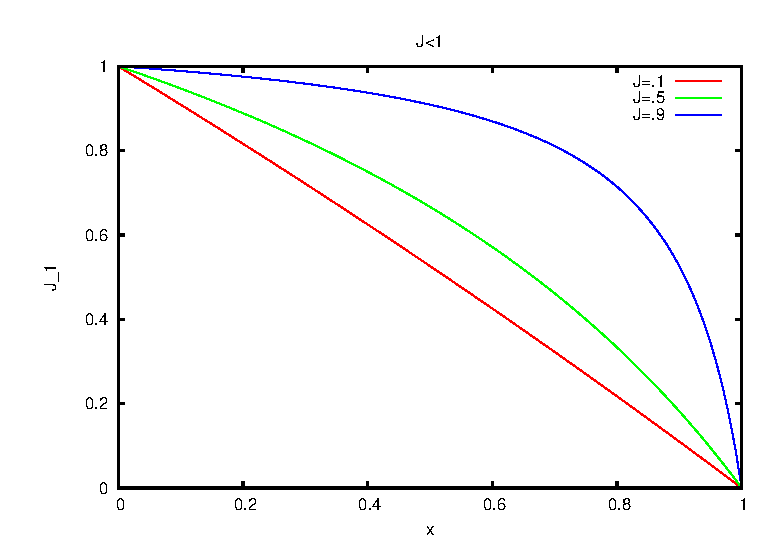
\includegraphics[width=.4\columnwidth,angle=0]{j_disordered.eps}
%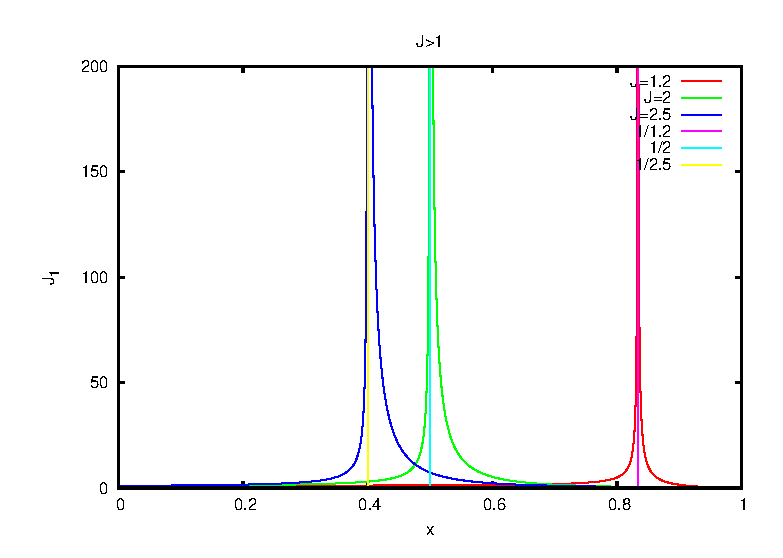
\includegraphics[width=.4\columnwidth,angle=0]{j_ordered.eps}
%\includegraphics[width=.6\columnwidth,angle=0]{jnew.eps}
%\caption{We plot the effective interaction as function of the unobserved nodes $x=N'/N$. In the left panel we show 
%the renormalization of effective coupling  $J<1$ when the total system is in the disordered phase while in the right panel 
%we are in the ordered phase $J>1$. In the former, increasing the unobserved fraction $x$ we flow with the RG to weak coupling: the bigger the fraction of unobserved nodes the smaller is the effective interaction between spins. In the latter instead, the fixed point is strong couplings and the coupling increases and has an asymptotic value around the critical fraction $x=1/J$. The net result of decimation is thus to follow the RG flow and the effective couplings appear to be renormalized except at the fixed point $J=1$ where the couplings are constant.}
%\label{fig:flow}
%\end{figure}
So all the couplings are renormalized and in particular whenever $\beta J x<1$ $\overline{m}=0$ so that the parity of the free energy is recovered $J_1=J_3=J_5=0$. Meanwhile the non null interactions reads
\begin{eqnarray}
J_2= \frac{J (x-1)}{\beta  J x-1} \qquad J_4=\frac{\beta ^3 J^4 x (x-1)^3 }{3 (\beta  J x-1)^4} \qquad J_6 = \frac{\beta ^5 J^6 (x-1)^5 x (3 \beta  J x+2)}{15 (\beta  J x-1)^7}
\end{eqnarray}
Let us discuss their dimensions as function of the renormalization parameter $b=1/(1-x)$. We know that above the critical temperature $\sigma_o=1/(b^{\omega}) \sum_{i=1}^{b} \sigma_i $. Since we have the gaussian fix point  where every variable is independent with null mean value and fixed variance $\Delta$, we have that $$\langle \sigma_o^2\rangle = b^{1-2 \omega} \langle \sigma^2\rangle $$ So that the dimension of the magnetization is $\omega=1/2$. In this regime when integrating over $b=1/(1-x)$ variables we get that $m_o \to m_o \sqrt{b}$. After rescaling $N \to N /b$, so in order to keep the energy invariant $\mathcal{E}_o \to \mathcal{E}_o$ we have that
$$J_2 \to J_2  \qquad J_4 \to  J_4 b \qquad J_6 \to J_6 b^2\,.$$
We thus need to define the renormalized running coupling constant removing the dependence of the dimension such that the adimensional coupling constant $J^a_2=J_2$ while $J^a_4=J_4 / b=J_4 (1-x) $ and $J^a_6=J_6 /b^2=J_6(1-x)^2$ that will be our
parameter. We can define the beta function for this quantities that is the log derivative in terms of the running constants. Concerning the two body interaction beta function
\begin{equation}
-\beta_2(J^a_2) = (1-x) \frac{\partial \log J^a_2}{\partial (1-x)} =-(1-x) \frac{\partial \log J^a_2}{\partial x} = \frac{\beta J -1}{\beta J x -1} = 1-\beta J^a_2 =
\end{equation}
so we get a fixed point $\beta J^a_2=1$. In the same way we get the four body interaction term
\begin{equation}
-\beta_4(J^a_2, J^a_4) = (1-x) \frac{\partial \log J^a_4}{\partial (1-x)} =-(1-x) \frac{\partial \log J^a_4}{\partial x} = \frac{\beta  J x^2+x (3 \beta  J-5)+1}{x (\beta  J x-1)}
\end{equation}
In terms of the adimensional running coupling constants we have that 
\begin{equation}
-\beta_4(J^a_2, J^a_4)  =   2 + 3(1-\beta J^a_2) - \beta J^a_2\left(1-\frac{(\beta J^a_2)^3}{3\beta J^a_4} \right)
\end{equation}
At the fixed point $\beta J^a_2=1$ we get that the $J^a_4$ has a fixed point at $-1/3$. 
Instead for the last coupling constant $J^a_6$ 
\begin{equation}
\beta_6(J^a_2, J^a_4,J^a_6) = 4+ (1-\beta J'_2) \left(5 + \frac{6}{5} \frac{(\beta J^a_4)^2}{\beta J^a_6 (\beta J^a_2)^2}\right)- 2\beta J^a_2 \left( 1+ \frac{1}{15} \frac{(\beta J^a_2)^5}{ \beta J^a_6} - \frac{3}{5}  \frac{(\beta J^a_2)^2 \beta J^a_4}{\beta J^a_6}\right) 
\end{equation}
In the opposite regime whenever $\beta J>1$, the system is in the ordered phase. In this region we have to distinguish the case $\beta J(1-x)<1$ and $\beta J(1-x)>1$.
In the first regime $\beta J(1-x)<1$, we can still expand the self consistent equation (\ref{selfconsistent}) around zero. This means that equation (\ref{renJ1hT}) is still valid through this region until $\beta J(1-x)=1$ and it is telling us how $J'_2$ is effectively renormalized as a function of $x$. We can see that now the ratio $J'_2/J$ is always bigger than one and it diverges when the critical threshold $x_c=1-1/(\beta J)$ is reached, $$\lim_{ x\to x_c^+} \frac{J'_2}{J}=+\infty\,.$$ This means that the effective coupling $J'_2$ is getting bigger and the system is flowing toward the strong coupling fixed point (see right panel in Fig \ref{fig:flow}). 


This analyses can not be pushed further when $x>x_c$ since this means $\beta J(1-x)>1$ and this regime the expansion of the hyperbolic tangent is not longer valid. When we approach the asymptote from right $x \to x_c^-$ we need to take into consideration the onset of a non null magnetisation in the hidden system $\mathcal{A}$.
\begin{equation}
m_0^2= \frac{3(Jx-1)}{(Jx)^3} \qquad \alpha=\frac{3-Jx}{Jx (Jx-1)}
\end{equation}
Substituting the solution $m^*=m_0+\alpha h$ in the free energy we get that
\begin{equation}
f(m_1,m^*)=-\frac{1}{2} J(1-x)^2 m_1^2 - \frac{1}{2} x(1-Jx) (m_0^2+2 \alpha J(1-x) m_0 m_1 + \alpha^2 J^2 (1-x)^2 m_1^2)
\end{equation}
Together with a non null average value, we get a renormalized coupling $J_1$ that reads
\begin{equation}
\frac{J_1}{J}= (1-x) \left( 1+ J x (1-Jx)\alpha^2 \right)= (1-x) \left( 1- \frac{(3-Jx)^2}{Jx(Jx-1)}\right)
\end{equation}
The behaviour is shown in the right panel of Fig. \ref{fig:flow}, where for $J\sim 1$ the error in the coupling is small and get bigger and bigger with the increasing of the real coupling making the system flow toward the strong coupling fixed point.

-What about spin glass in mean field?
-What about dimensional system with known RG fixed point?
\begin{figure}[h]
%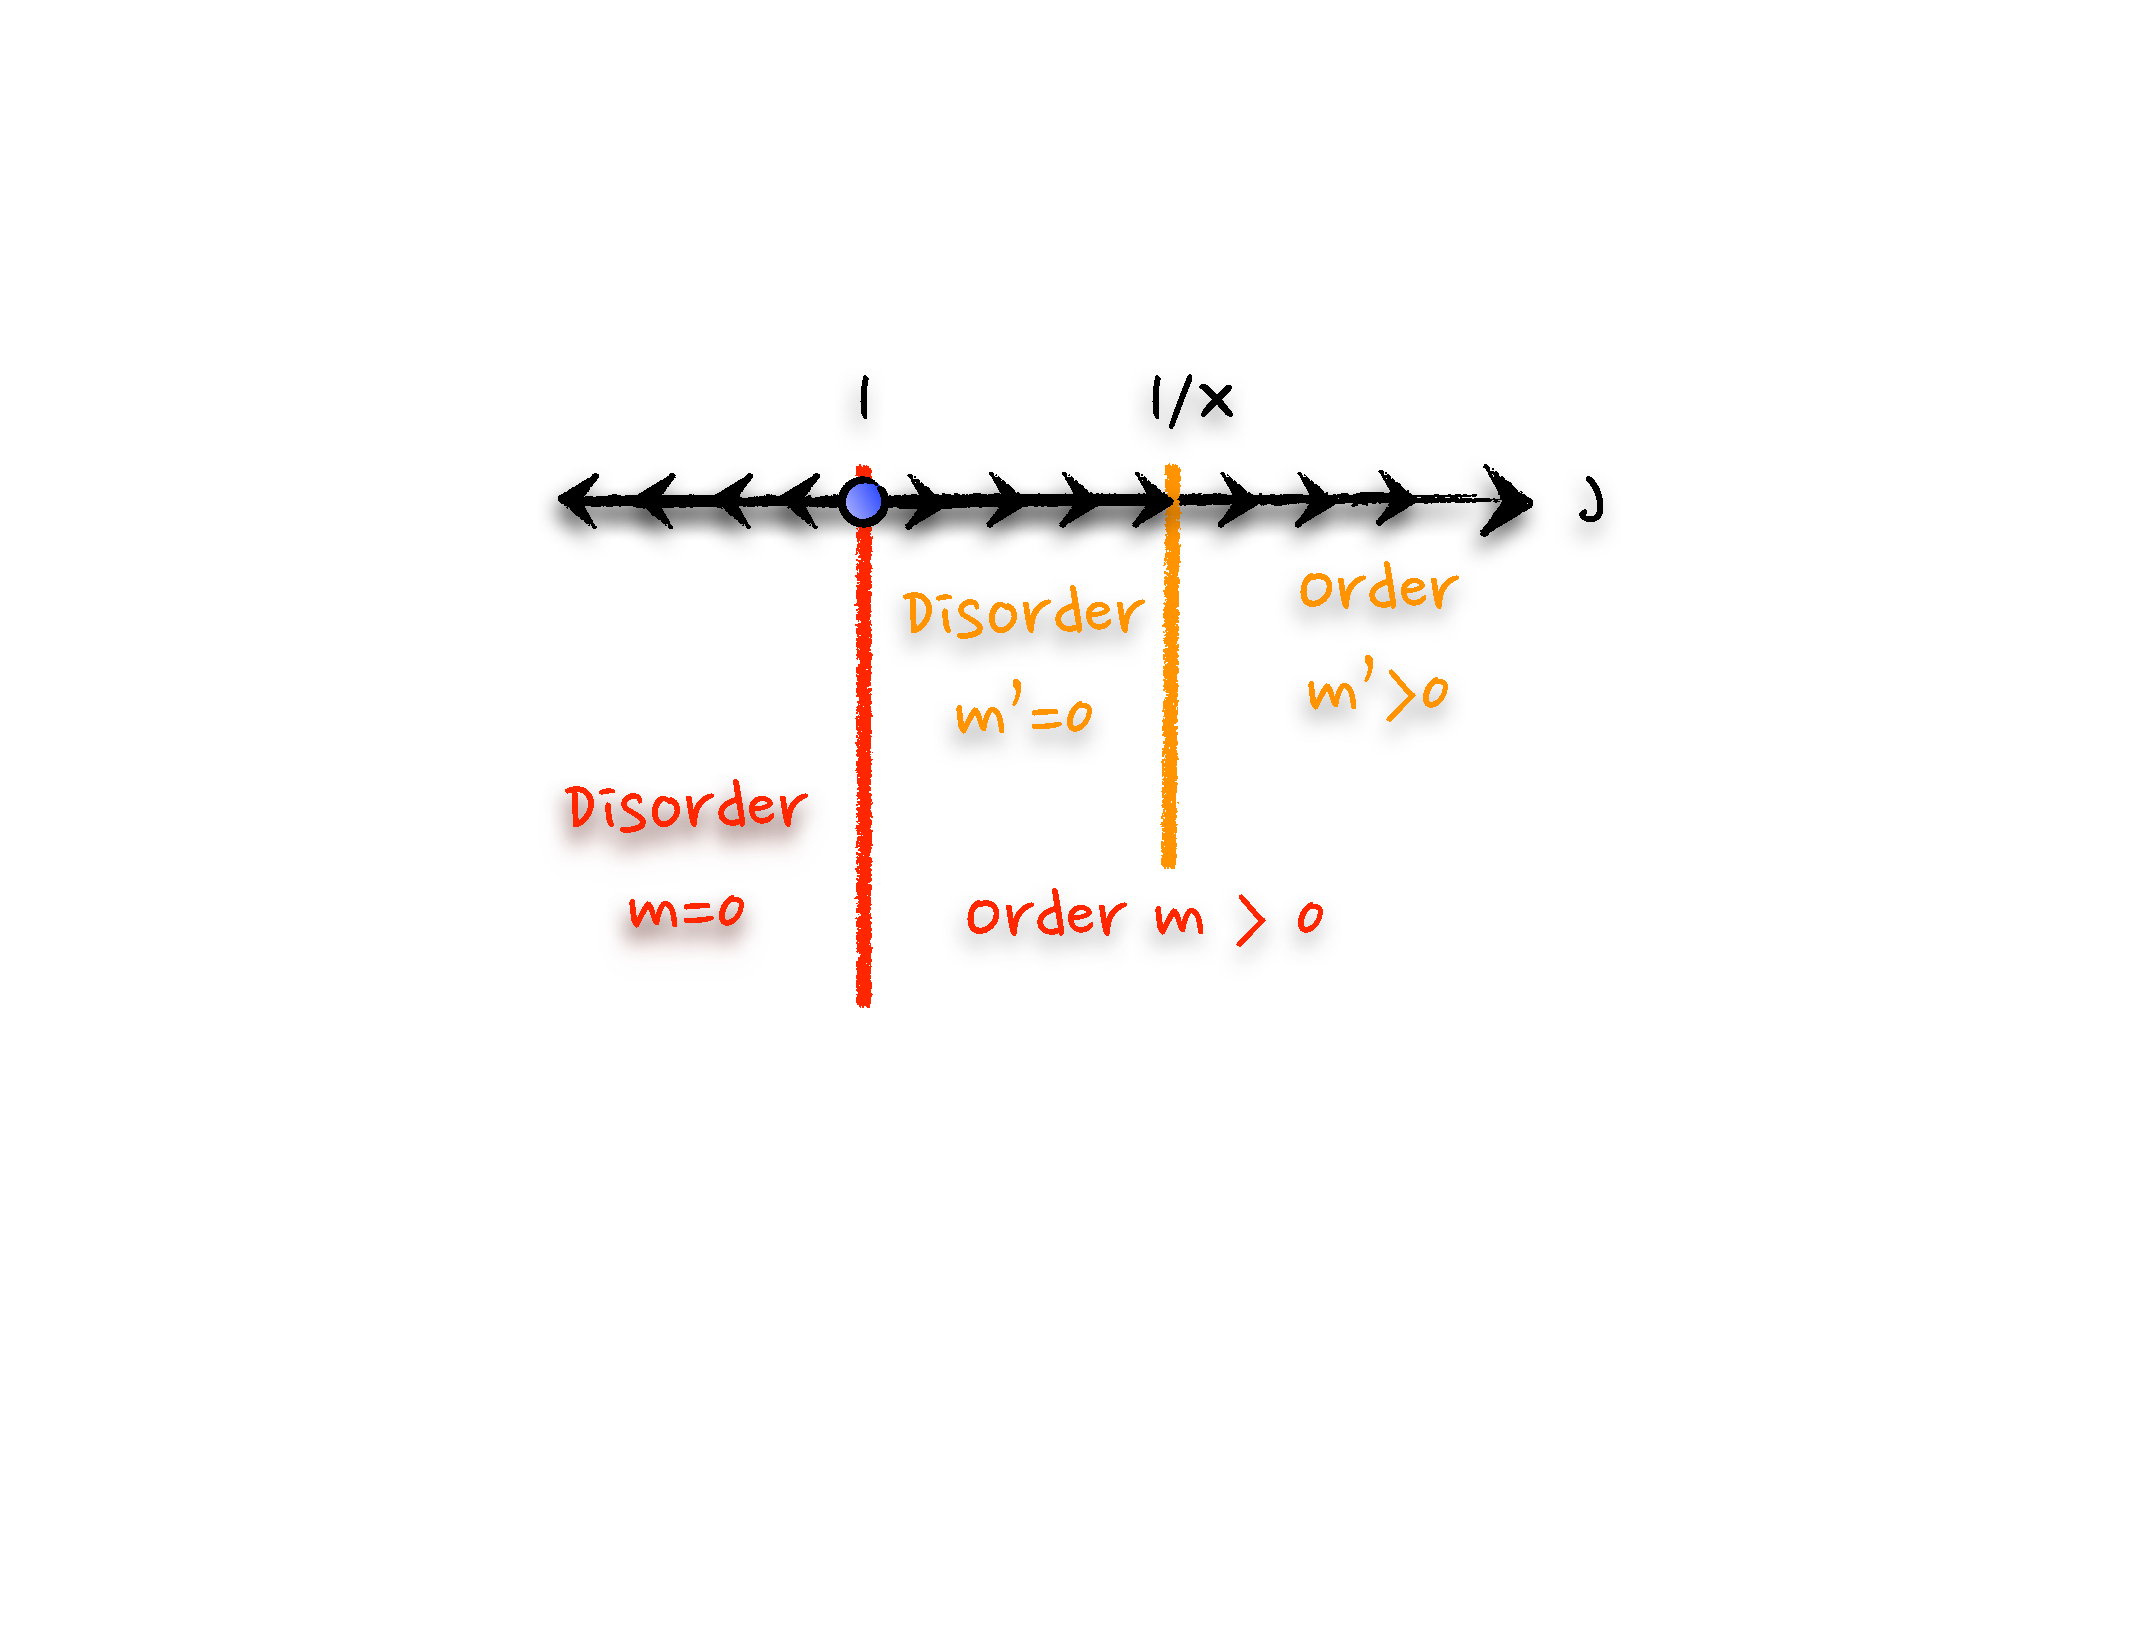
\includegraphics[width=.5\columnwidth]{phasediagram.pdf}
\caption{In figure we sketch the phase diagram of the system as a function of the parameter $J$. If $J=1$ the system is not renormalized by the decimation procedure. Interestingly, when $J<1$ the system flows to the high temperature fixed point while
for $J>1$ we get that the system is going to the strong coupling regime. It is important to emphasize that although the two subsystems may appear to have lower critical temperatures, they know to be in the ordered phase and the effective coupling gets stronger and stronger increasing the fraction of unobserved nodes $x$.}
\end{figure} 
\end{document}